In this section we are going to show some mockups of the system regarding the mobile application. On the RASD document we have presented some web application mockups and how they can be derived from mobile ones; for this reason we suppose UI developers will be able to derive correct web application mockups from the following ones.\\
During the design of mockups we have followed exactly the structure that is presented on UX diagrams; we won't show all the screens that are on the UX diagrams, however a lot of them have been created trying to clarify precisely how the user should interact with the system.\\
The mockups we are going to present are the following:
\begin{itemize}
	\item \textbf{Homepage}: This mockup shows the external homepage of the system. This can be seen by anyone who downloads the application and want to register or login.
	\item \textbf{Calendar Page}: In this mockup we show the main page of the system where users are able to seen their meetings and travels. We offer the possibility to easily switch between daily, weekly and monthly views and create a new meeting. Moreover we show the meeting and travel details page where users can see in detail their events.
	\item \textbf{Notifications}: We have designed a notification page where a warning and an invitation are pending. The user can click on warning to open the overlapping meetings page where it can accept, decline or reschedule each of them; a rescheduling proposal page has been designed too. In addition, the user can choose to see in detail the meeting to which it has been invited.
	\item \textbf{Settings}: This mockup shows the current status, the current default location and daily breaks. We have designed also a page where the user can edit its preference list, marking travel means that it doesn't want to use as inactive. Moreover we have created mockups related to the process of adding a new constraint. The system suggests the user all the possibilities it can choose from while creating the new constraint.
\end{itemize}

\begin{figure}[h]
	\centering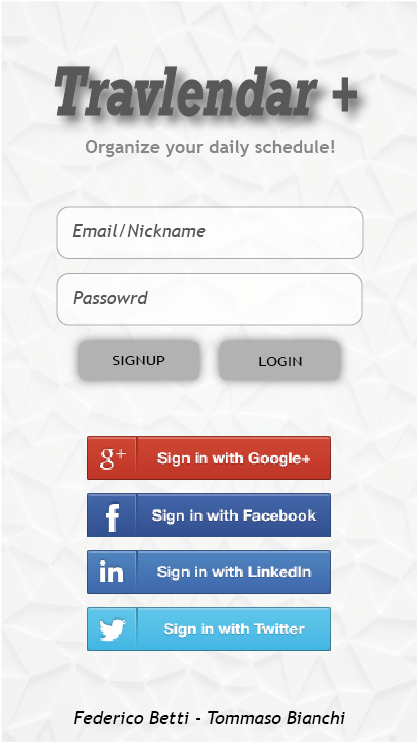
\includegraphics[scale = 0.35]{Images/Mockups/HomePage.png}{}
	\caption{External Homepage}
\end{figure}

\begin{figure}[h]
\centering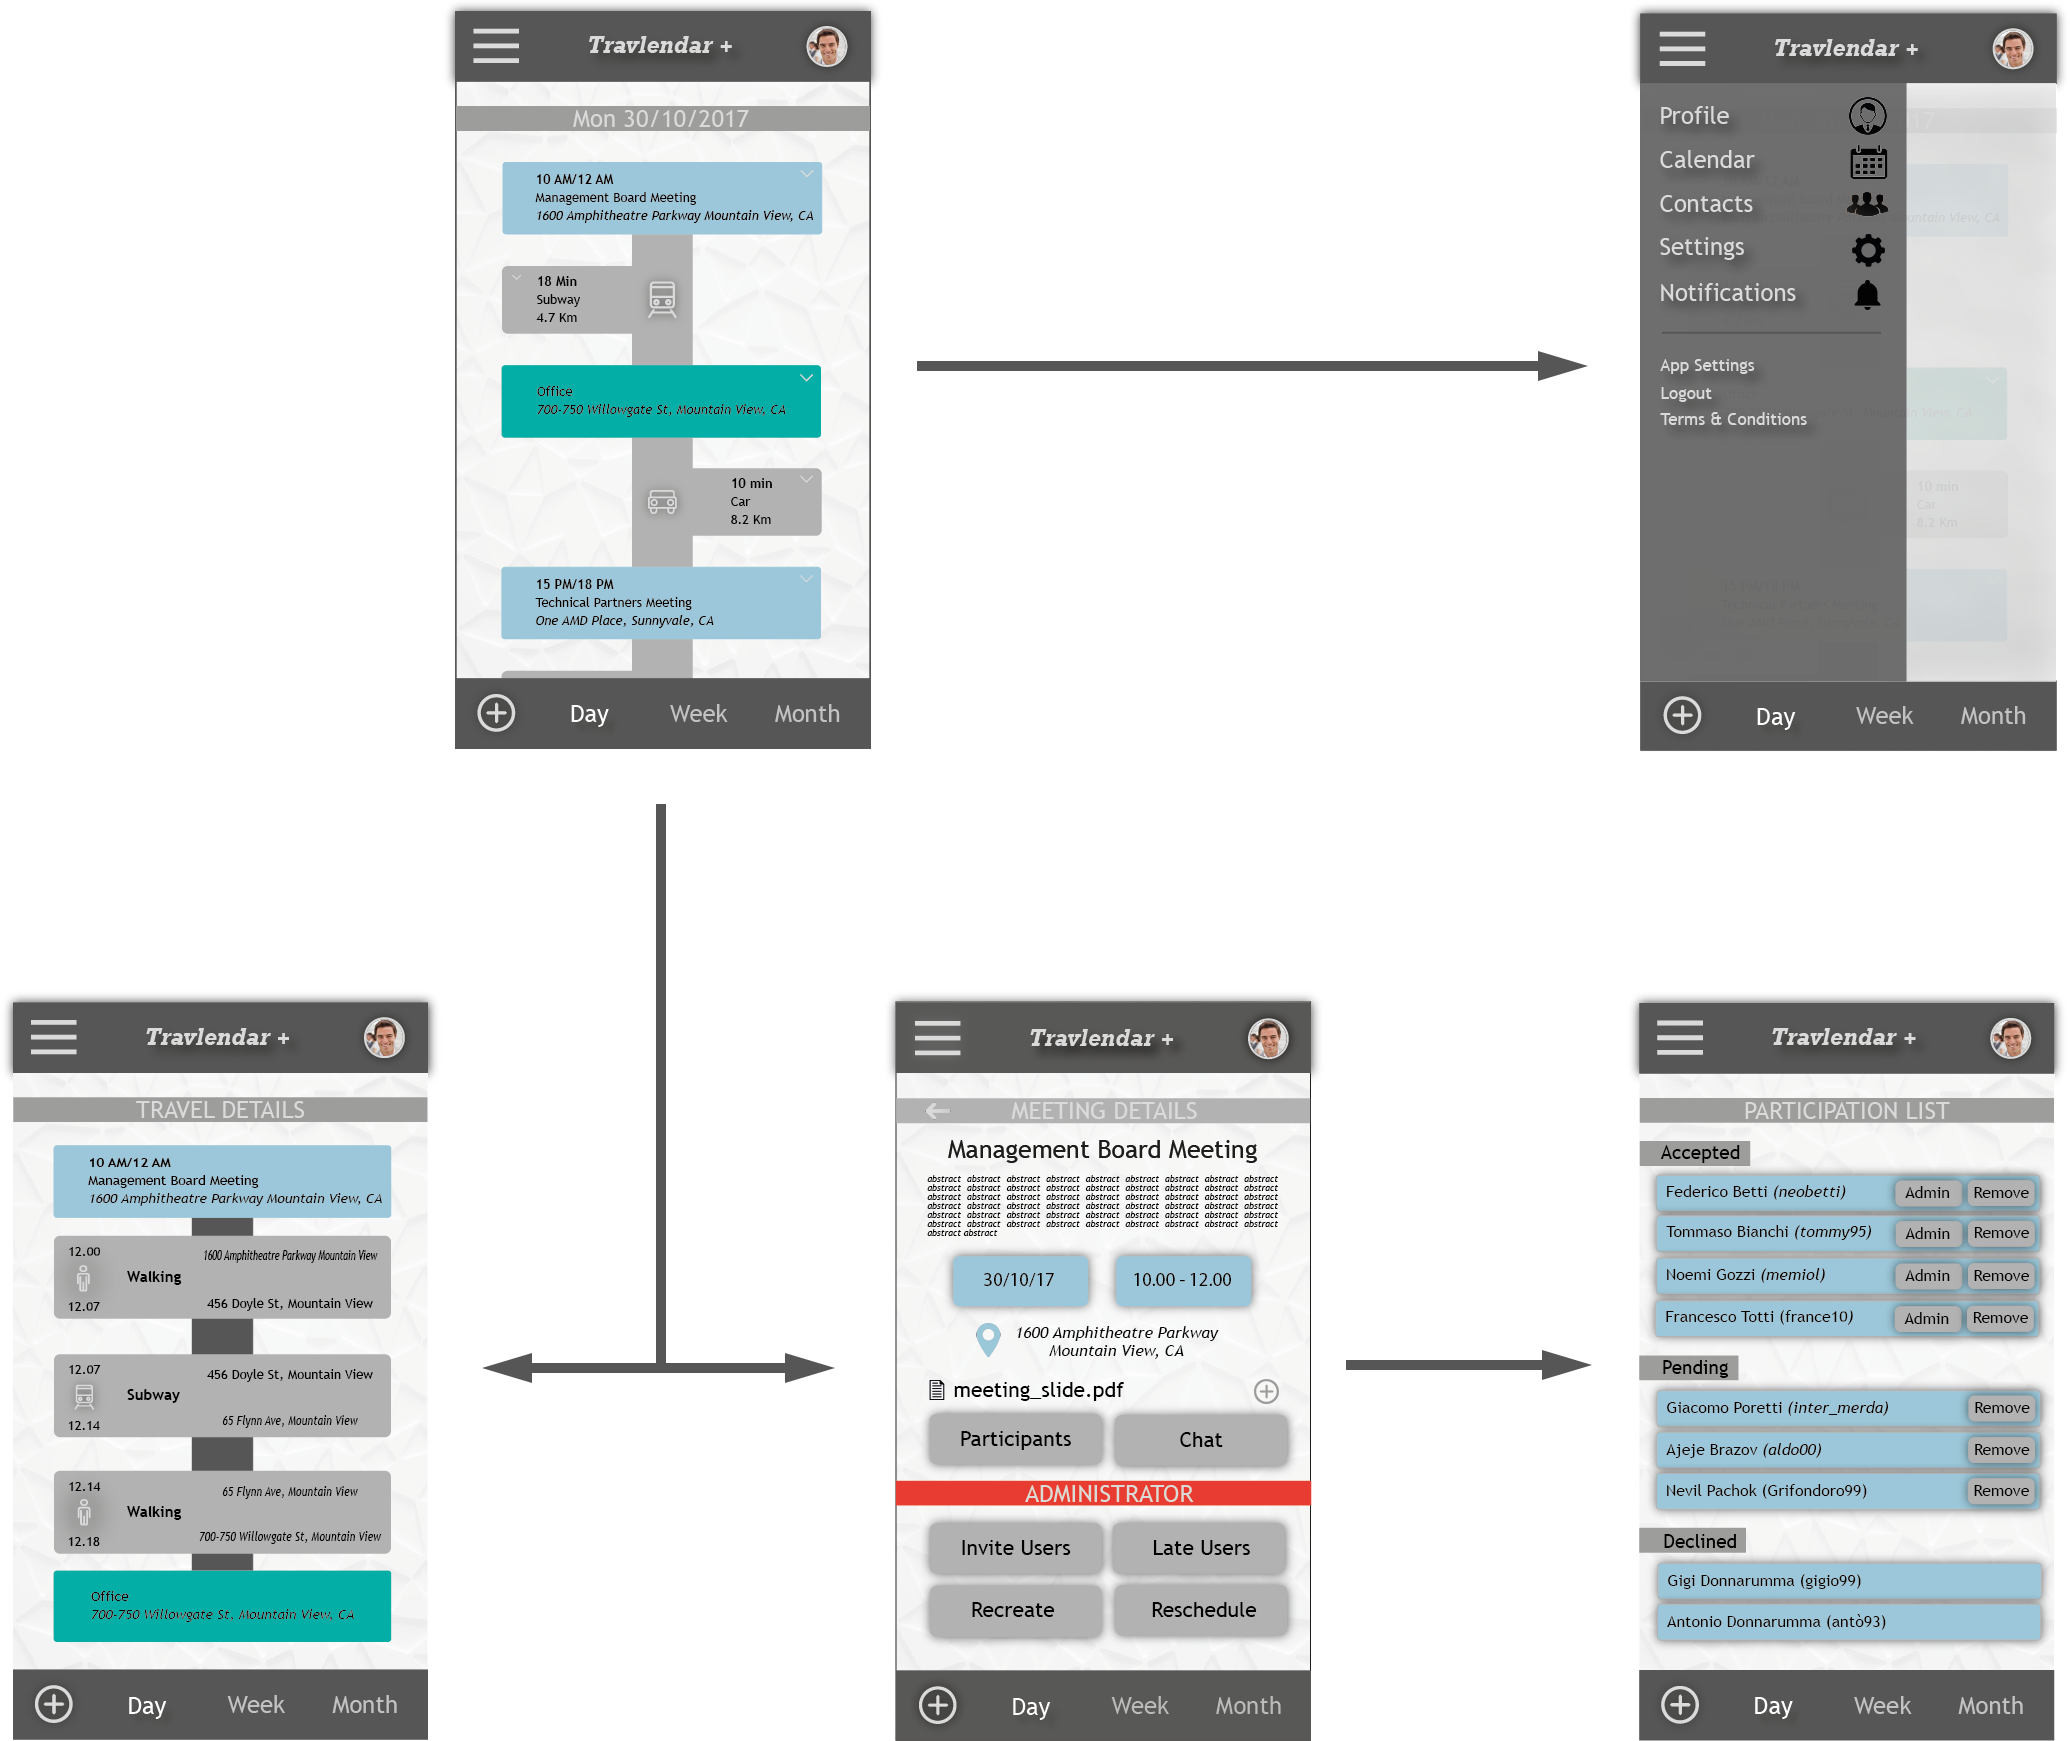
\includegraphics[width = \textwidth, scale = 0.3]{Images/Mockups/CalendarPage+.png}{}
\caption{Calendar Page Mockup}
\end{figure}

\begin{figure}[h]
\centering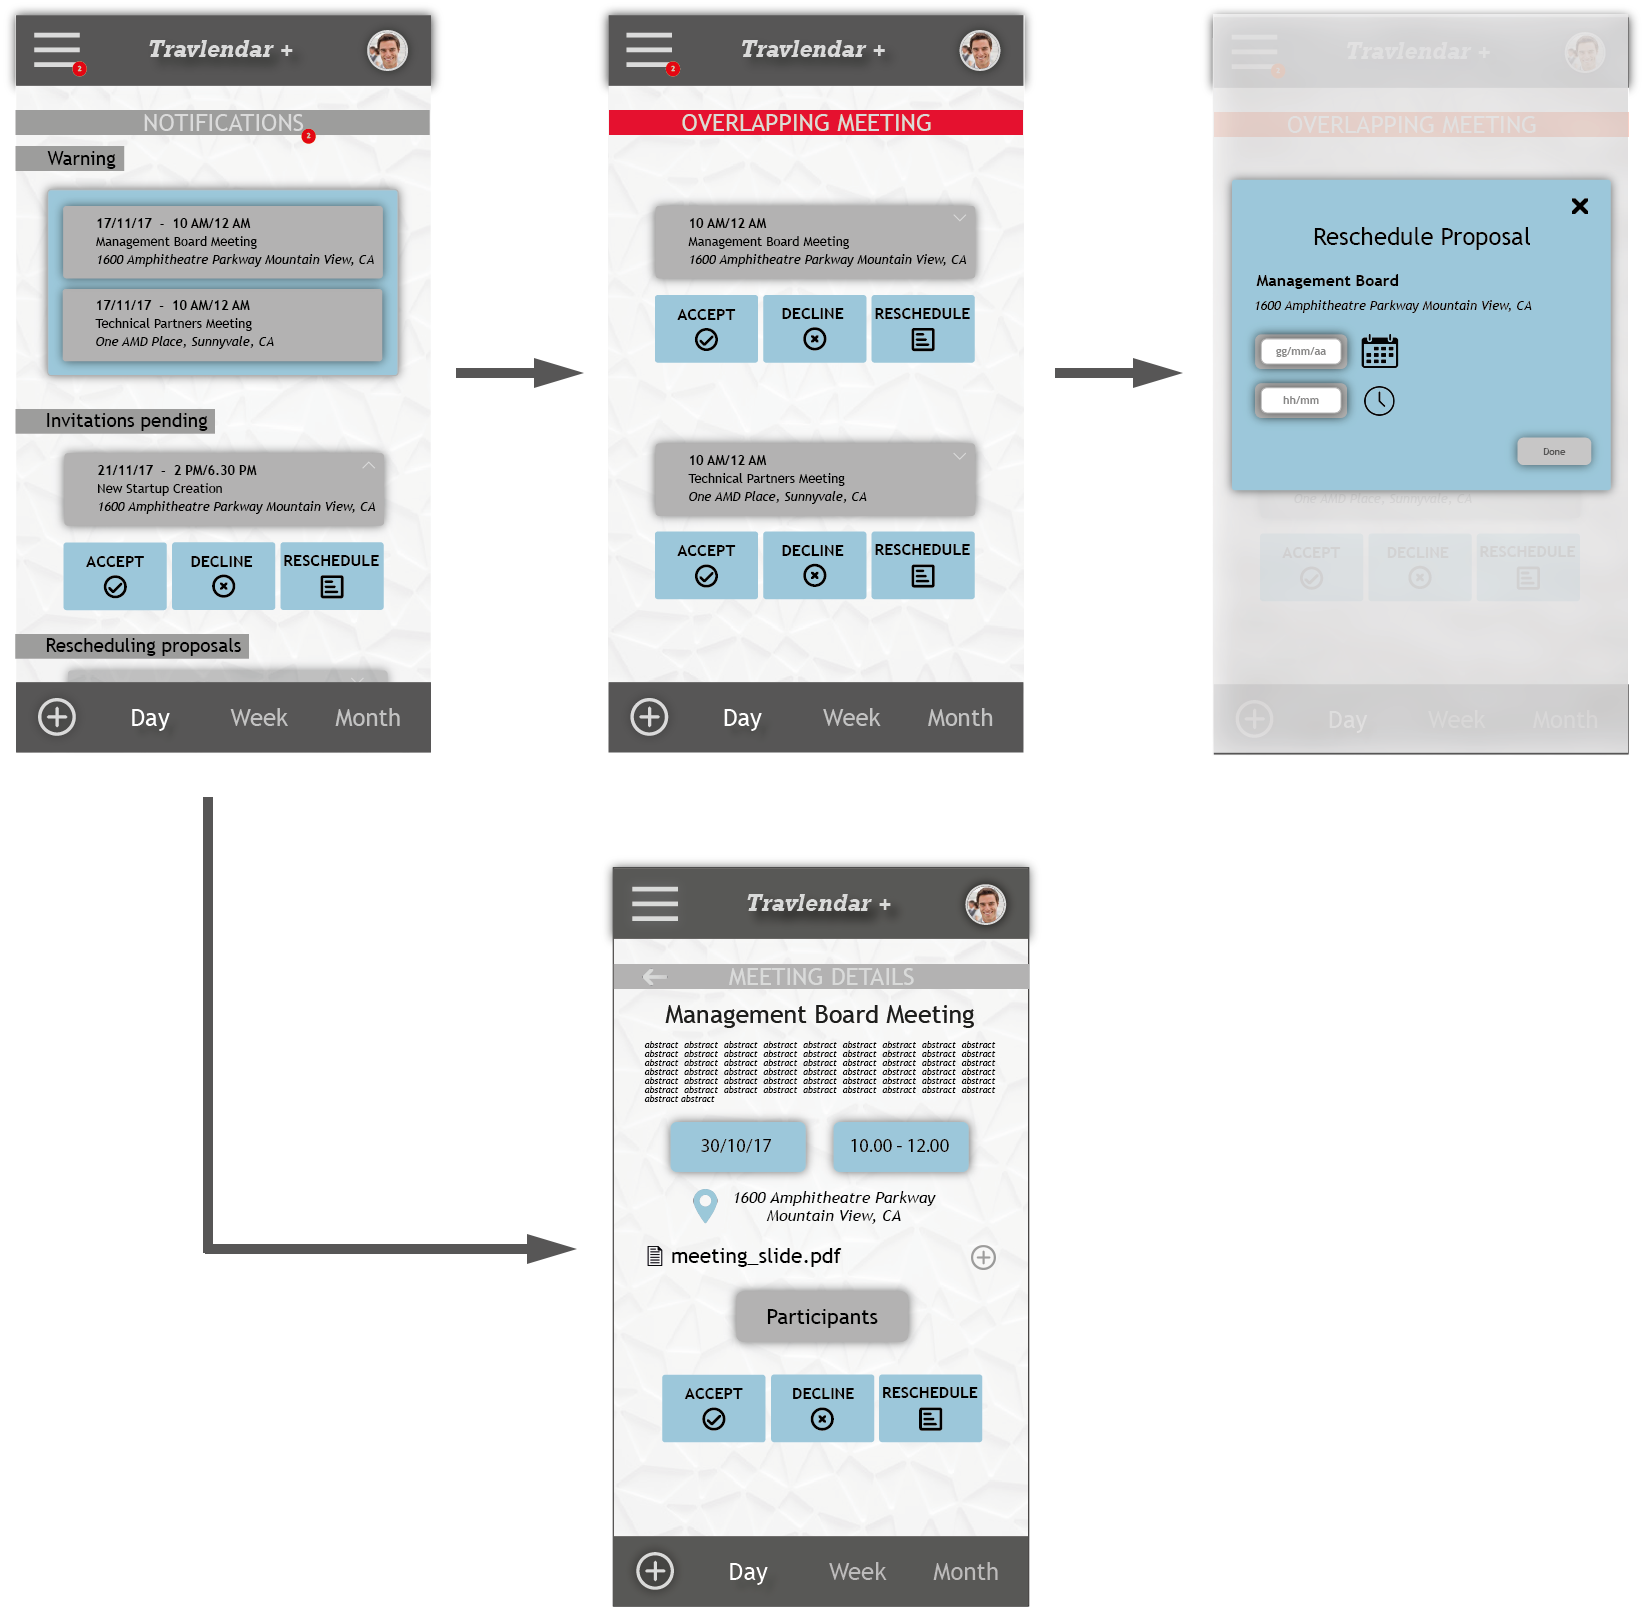
\includegraphics[scale = 0.3]{Images/Mockups/Notifications+.png}{}
\caption{Notifications Mockup}
\end{figure}

\begin{figure}[h]
\centering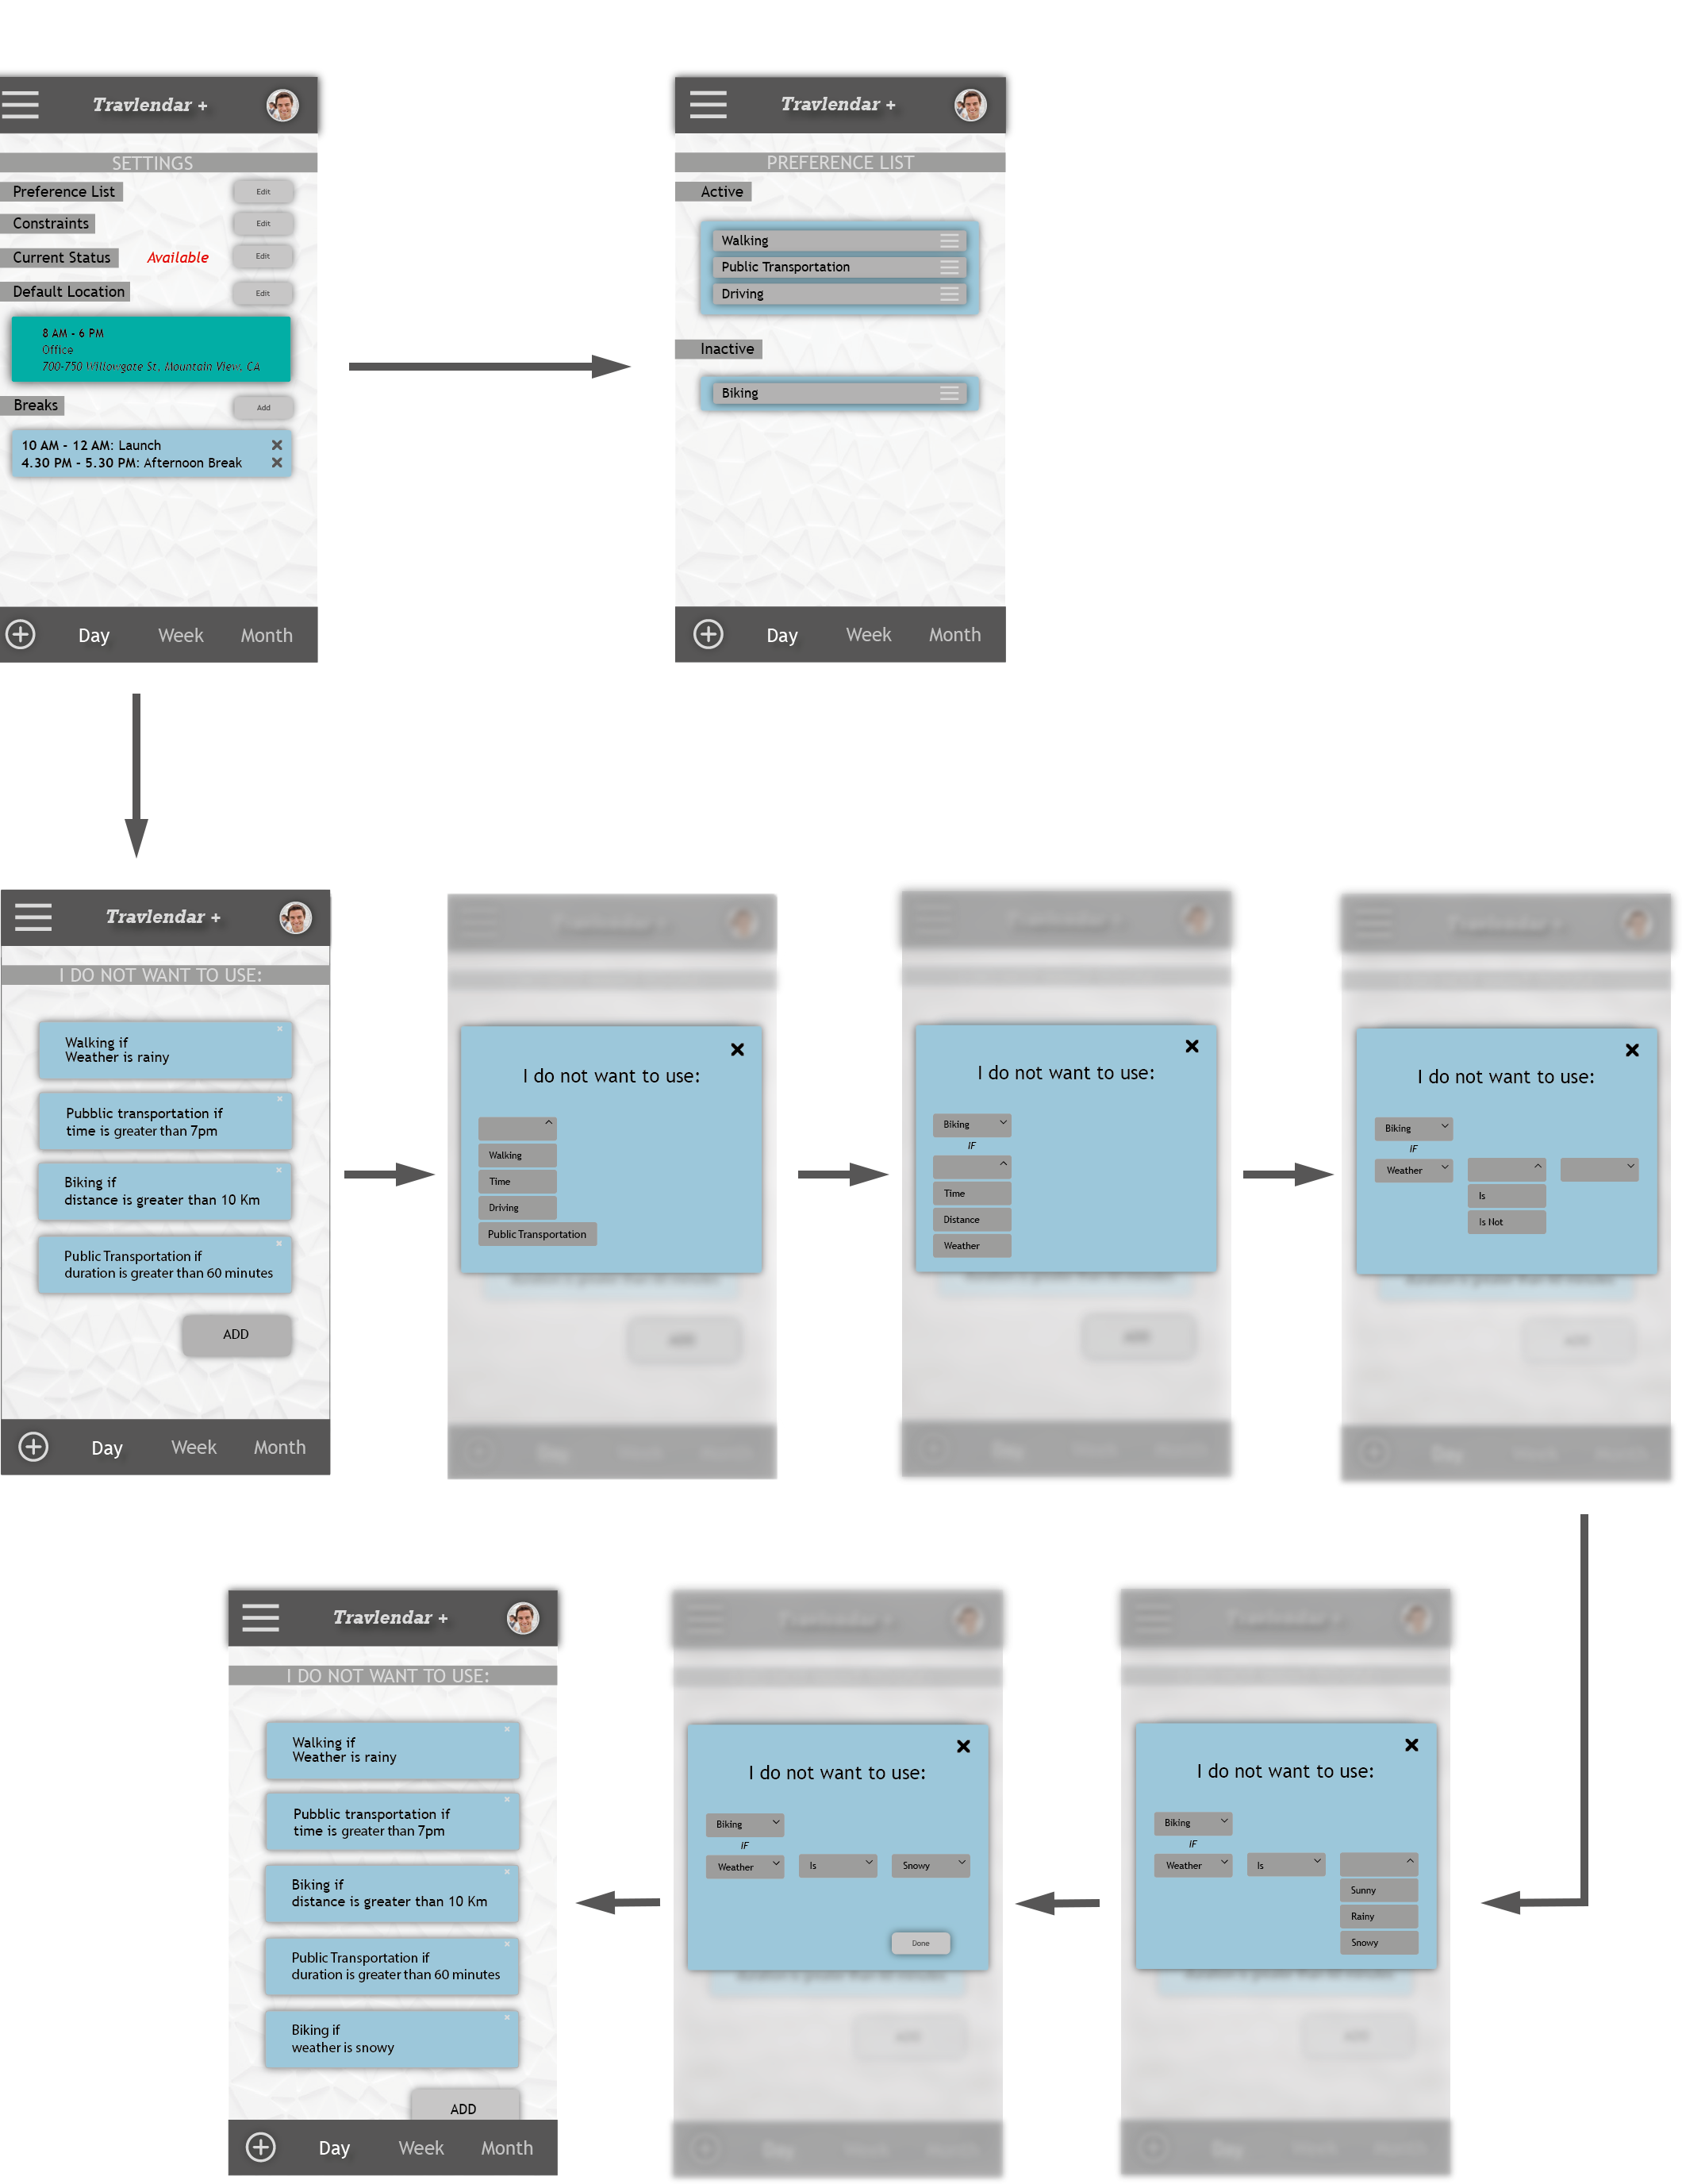
\includegraphics[width = \textwidth, scale = 0.3]{Images/Mockups/Settings+.png}{}
\caption{Settings Mockup}
\end{figure}
\clearpage